\chapter{Ripple Attacks}
\label{attack}

\section{Motivating system: Artificial Pancreas System}


We use a DNN based \ac{APS}, closed-loop model, by Dutta et al. \cite{10.1007/978-3-319-99429-1_11}  as our motivating example for illustrating a \ac{RFDIA}. 
We use this to explain our motivating attack. 
The \ac{APS} model we use in this section is also our first evaluation system; it is also the simplest of the three systems in terms of \ac{DNN} complexity described in ~\ref{dnncomplexity}.
A patient relies on  \ac{APS} to correctly determine the next dose of insulin to be injected every $t$ minutes. 

\begin{figure}
	\centering
	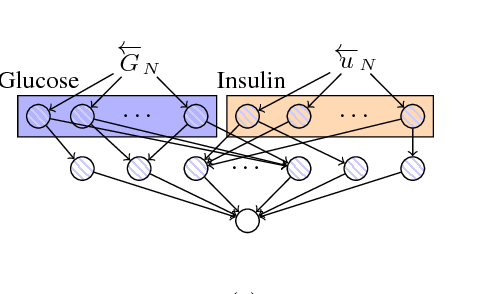
\includegraphics[width=0.7\linewidth, height=0.3\linewidth]{Images/APSDNN}
	\caption[APS DNN]{APS DNN designed by Dutta et. takes in 74 inputs of insulin and glucose. The next layers form connections between the insulin and the glucose to make predictions.[8]}
	\label{fig:apsdnn}
\end{figure}

%How is APS constructed?
The APS architecture is explained in Section ~\ref{apsdnn}. 
We examine the \ac{APS} controller model from Dutta et al., which has a feed-forward architecture. 
The DNN for APS creates mappings between the insulin and the glucose values that allow for the prediction of future insulin values as shown in Figure ~\ref{fig:apsdnn}. 
The insulin and the glucose values are the values collected from the sensors and the actuators. 
The model has 74 inputs in total, where 32 inputs are the glucose, and the other 32  are insulin values collected every 5 minutes.
 The DNN layers use these values as inputs to predict the next value. 
 This implies that the future value is predicted based on the inputs from the previous set of values. 


%Defense mechanisms
There are two phases in a \ac{DNN}s life; training phase and inference phase. 
During the training phase, there are three \ac{DNN}s that are trained in an \ac{APS} to predict the next outcome. 
The first \ac{DNN} is used to predict the next outcome. 
The accompanying two \ac{DNN}s are for the purpose of designing defense mechanisms such that the patient is not overdosed with insulin.  
The two \ac{DNN}s are separate from its main decision making controller. 
These \ac{DNN}s are trained based on the latest 30-day patient data which is collected from monitoring the patient, to understand the standard injections for a patient over time. 

One \ac{DNN} learns a lower threshold on injection amount; the other learns an upper bound on injection amount. 
Hence, for every time of the day based on the previous patient characteristic, the minimum and the maximum values are known. 
However, the system will not detect  an adversary  who manages to always administer the maximum allowed dosage through \ac{RFDIA}. 
Hence, the attacker needs to identify inputs and  perturb them  such that the output changes the maximum allowed dosage for every injection,
  while being lower than the upper threshold to avoid detection, and cause maximum potential damage to the patient. 


\section{Attack Model}
The attacker's goal is to manipulate the sensor measurements to conduct FDIAs without triggering alarms as shown in Figure ~\ref{fig:attackmodelphysical}. 
The attacker can use network noise or physical means of sensor tampering to attack the systems ~\cite{10.1145/3319535.3339815}.
 
\begin{figure}
	\centering
	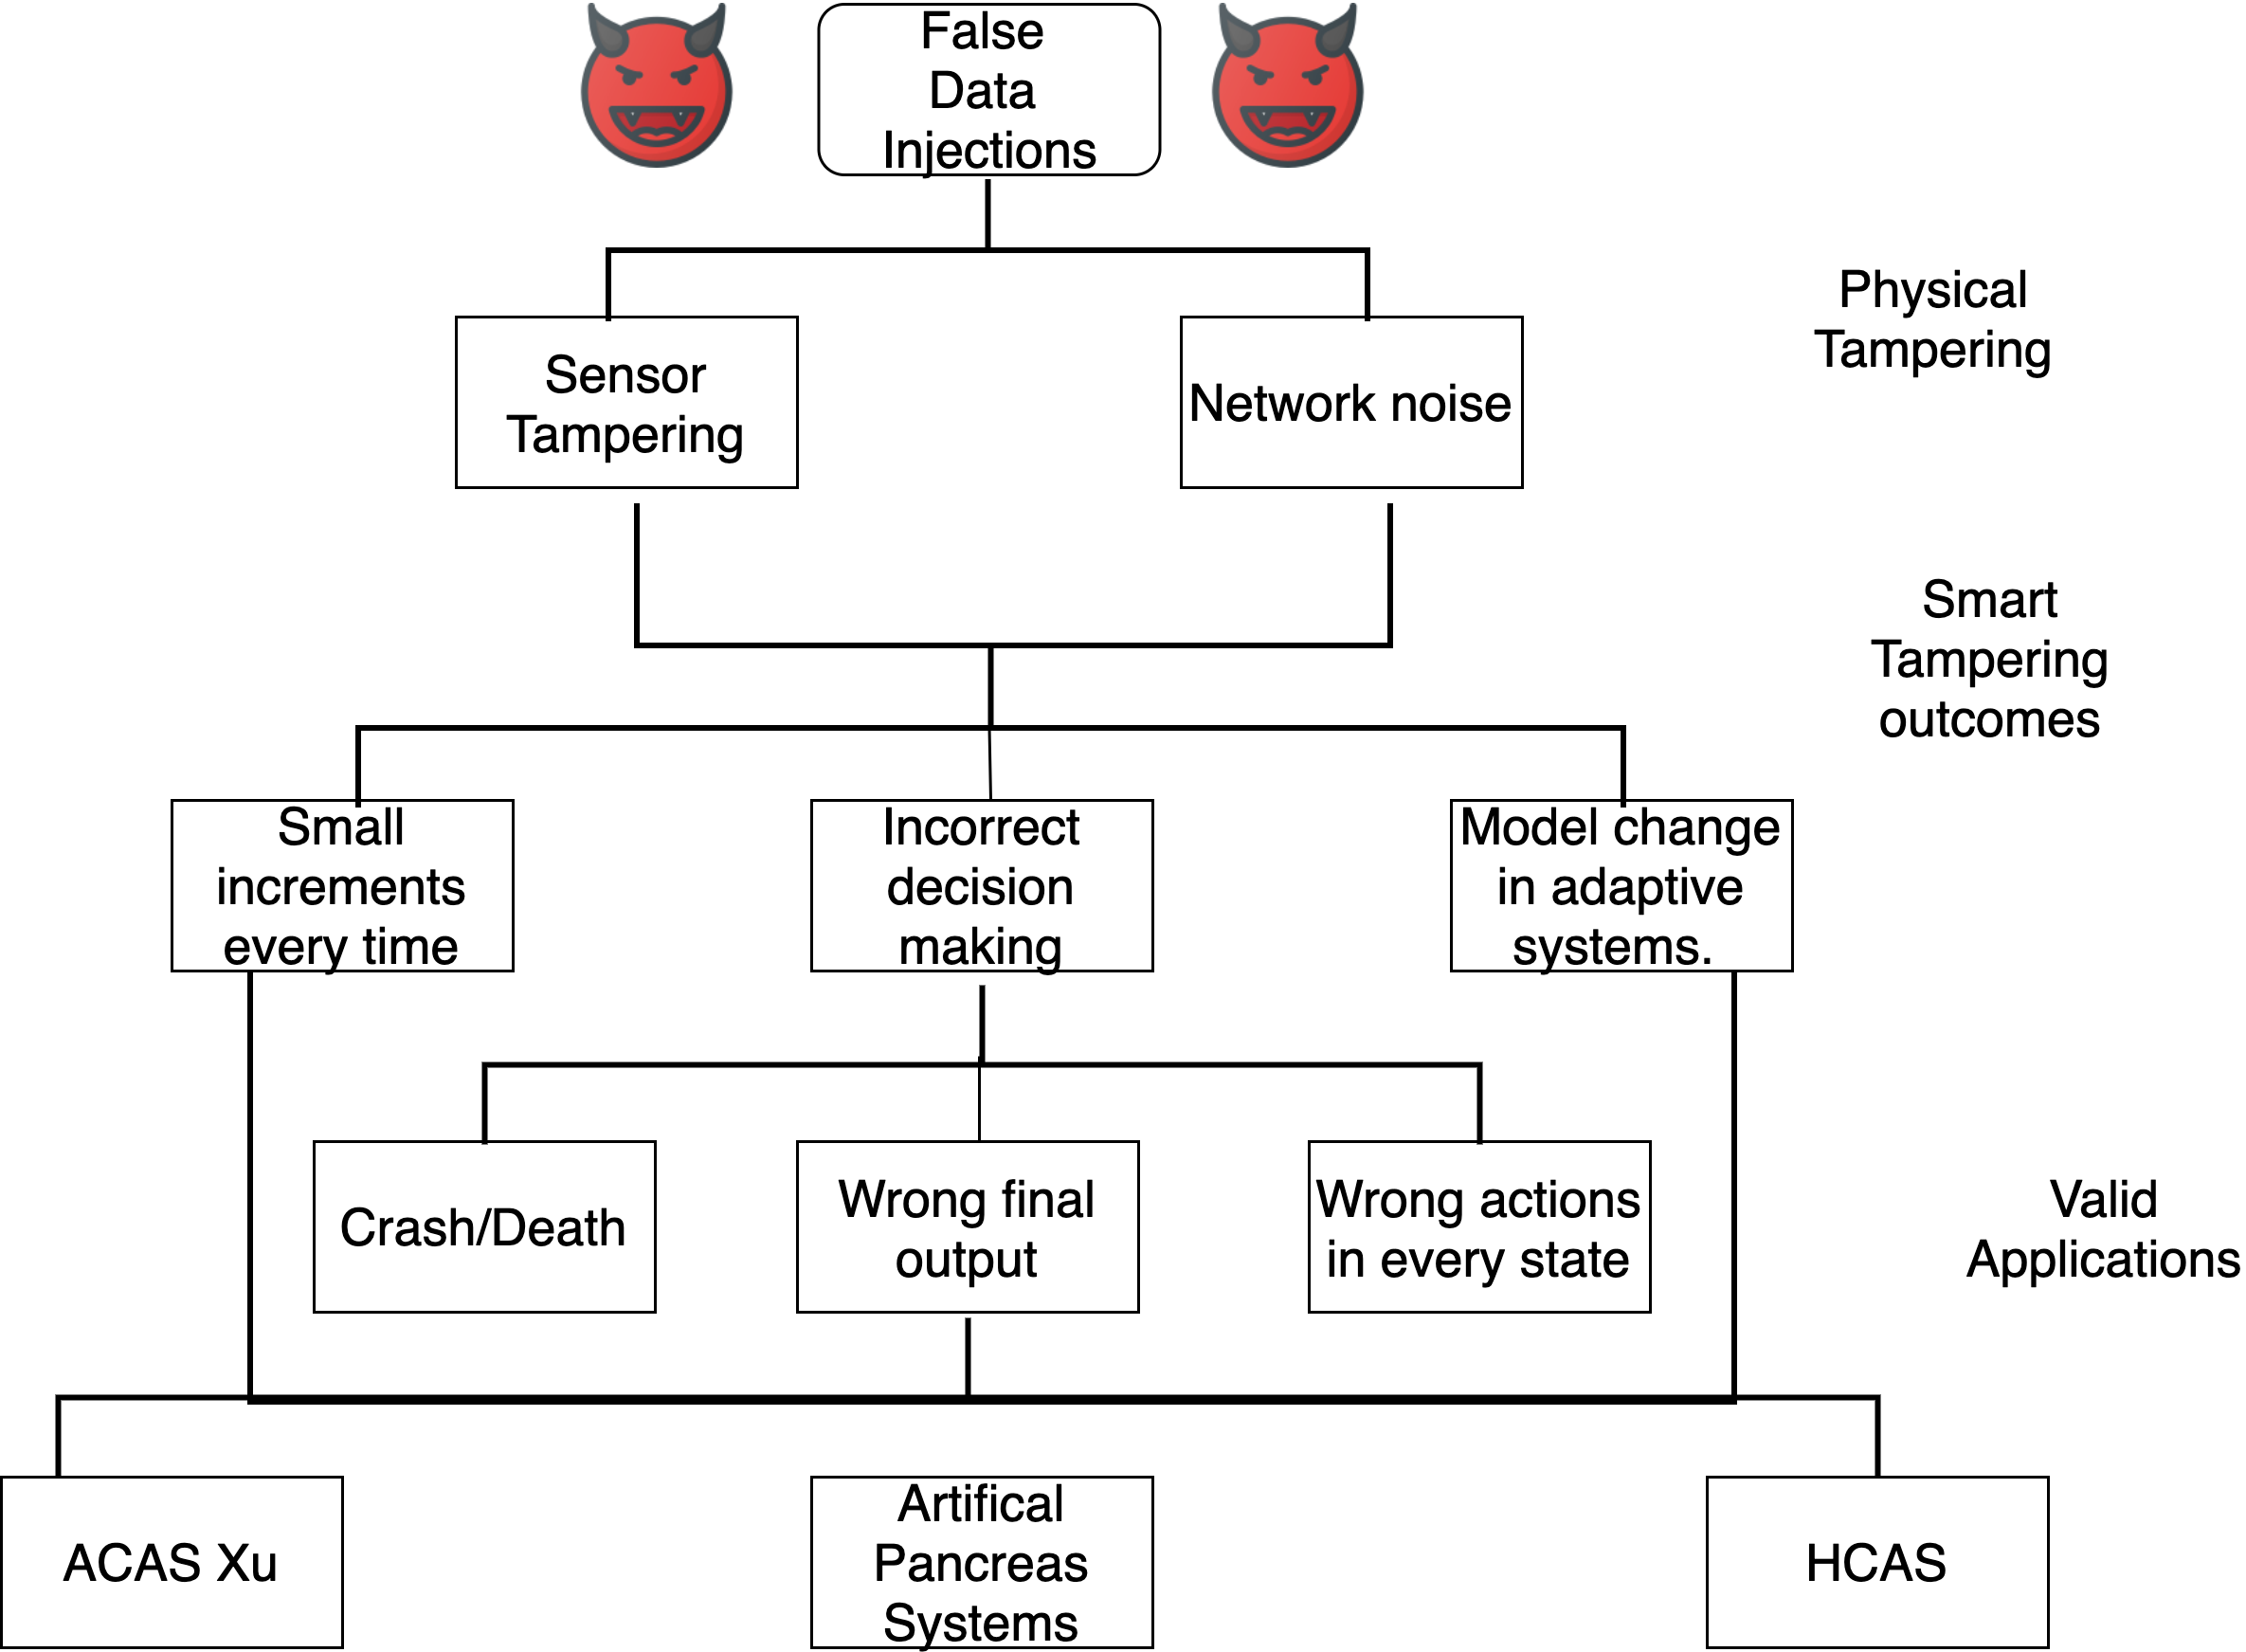
\includegraphics[width=0.7\linewidth]{Images/Attackmodelphysical}
	\caption{Attack model}
	\label{fig:attackmodelphysical}
\end{figure}

We assume that the attacker has following capabilities:
\begin{enumerate}
	\item The \ac{DNN}  architecture  is known to the attacker for example., a feed forward  network in case of an \ac{APS}. This information easy to find, as the architectures are  usually public information for the systems. 
	\item  The weights and bias of the \ac{DNN}  architecture are known as well through a read-only access to the system.  
	\item The attacker cannot modify the code of the system, but can modify the inputs to the model.
	\item The \ac{DNN} contains ReLU as its activation function. %All three systems in this work contain ReLU.
\end{enumerate}

\subsection{Strawman attacker}
A simple way to attack the system would be to change all the 74 values that are the inputs to the DNN.
 If all the inputs are changed, the final output prediction is going to be wrong. The problem in this particular scenario is that 
 these inputs are collected every five minutes from the sensors attached to the patient. 
 This means that the attacker will have to conduct FDIAs every five minutes when the data is being collected, to cause a change in the output. 
 However, this is quite tedious in a practical scenario and hence, the attacker needs a better way of attacking the system. 

\subsection{Sophisticated Attacker}
A more sophisticated approach to attack the system would be by perturbing one or two inputs out of the 74 inputs that cause a change in the output. There are two ways to proceed when the attacker tries to change just one or two inputs at a time. 

\subsubsection{Attack 1}
The attacker can randomly choose two inputs and perturb them by huge amounts. 
This will indeed cause a wrong output prediction. 
However, if the input is perturbed by large amount, the error detection mechanisms will recognize that there is an anomaly. 
To prevent this the attacker can choose to perturb the two inputs by small amounts. 
However, perturbing any two random inputs by very small amounts might not necessarily lead to a wrong output prediction as shown in Chapter ~\ref{evaluation}. 

\subsubsection{Attack 2}
Adding one more layer of sophistication, the attacker does not
know the critical inputs or the input whose perturbation can lead to wrong predictions.
 This will be a more targeted approach for attacking the system since the input selection will not be random. 
However, not knowing the precise amounts by which the critical inputs should be perturbed can lead to an unsuccessful attack. 
If the perturbation is too high, it will trigger the error-detection mechanisms, 
and if it is too low, it will not affect the output as shown in Chapter ~\ref{evaluation}. 

\subsubsection{Attack 3}
The most sophisticated means for an attacker to attack the system would be to know precisely which inputs to perturb and by what amounts,
 such that the output prediction is wrong. 
To do so, the attacker needs an automated technique that in limited time, finds the critical inputs
 and also the smallest possible perturbations that can ensure a wrong output prediction. 

%Our motivation for designing the technique were these different ways of attacking the system that can automatically synthesize attacks in an efficient way. 

\chapter{Challenges}
We face  the following challenges during  the design of the technique. 

\section{ Mapping DNNs to MILP}
What do I want to say ?
- DNNs when with brute force take time since we cannot keep solving every solution space. 
- Define DNN solution space mathematically
- 
DNNs are complex algorithms 
It is is difficult to use b


\section{\textbf{C1}: Finding the critical inputs}
For the sophisticated attacker to conduct \attack as described in Chapter 3, the attackers require two vital pieces. The first one is finding the critical inputs. We explain this with our motivating example of the APS system from Chapter 3. APS has 74 inputs. It is not feasible to change all inputs by False Data Injection since the attacker will have to keep changing the inputs every five minutes. Therefore, if the model architecture is known to the attacker, the goal of the attacker is to quickly locate the critical inputs. Given this is a DNN based system, it is not possible to test it for every possible input-output combination in minimal amount of time to figure out the patterns for finding the critical inputs. 

\subsubsection*{Selecting  the automated technique}
The first part is choosing a technique that allows the attacker to model a DNN and find the critical inputs through the modeling. There are multiple means of modeling the DNN, some of which are using SMT solvers, symbolic execution, MILP and many more. 
Our goal is twofold: 
\begin{enumerate}
    \item generality
    \item scalability
\end{enumerate}

APS has a  feed-forward architecture with 74 inputs whereas the other systems on which we test our technique have completely different architectures as can be observed from Table 6.1 in Chapter 6. This is due to the difference in the application domain. APS is a medical system that is much easier to reason about as compared to our other test systems that are collision avoidance systems for air traffic control management.
APS has two layers and is the smallest system that we tested our technique for but we want our technique to be valid for much bigger systems as shown in Table 1. We show that MILP fulfills these two criteria by providing us generality and scalability. 


\section*{\textbf{C2}: Finding the input perturbations}
After locating the critical inputs, the next part of the challenge is to find the correct perturbations that can lead to ripples in APS. Based on Section V formulation, if the inputs in equation (1) ($x$) are perturbed by very small amounts, the effects are not observed in the final output due to the existence of K layers in the system and the ReLU activation function as shown in (3). There is not a linear mapping between the inputs and the outputs and hence, it is a challenging problem to find just the right perturbations. We show how we tackle this in our methodology using MILP. To find the correct perturbations for \attack, we run into the following challenge. 

\subsubsection*{Designing \attack specific cost function and selecting the range intervals for inputs and outputs. }
APS DNN is an architecture where K (the number of hidden layers) is 2, and the vector input $x$ consists of 74 inputs. Our attack model is that we want to perturb the inputs by the least amounts and cause deviations in the output that are not above a certain threshold. The threshold value is determined based on the specifications of the system as described in Section III. 
 Hence, our challenge here is how we design our cost function and add a range limit to the perturbations to ensure that the perturbation does not exceed the input values above or below the bounds. 















